\chapter{Combinatorial Optimization and Max-Cut}
\label{chap:combop}

Combinatorial optimization is about finding the optimum (either a maximum or minimum) of an objective function whose domain is discrete, but often very large. Examples of problems considered are the travelling salesman problem \cite{TSP} important in routing, and the knapsack problem \cite{Knapsack1,Knapsack2} that is a generalization of the struggle you face when you pack your bags for your holiday. Many other problems from day-to-day life, industry and science can be formulated as combinatorial optimization problems. However, exhaustive searches of the domain are ordinarily not tractable. For example, when packing your bag with $N$ items, you have an exponential number of combinations to choose from, namely $2^N$. Hence we need smart approaches if we want to tackle these problems. Sadly, even our smartest approaches are sometimes not enough to find optimal solutions efficiently. Instead, we can use approximation algorithms that find good solutions instead. These are algorithms that find for solutions that are as least as good as the optimum value times a certain factor, called the approximation ratio. Sometimes a good solution is all we can ask for.

In this chapter I will show some relevant problems encountered in combinatorial optimization, and explain the need for approximation algorithms. Furthermore, I will explain the Max-Cut problem in more depth together with its applications. Next, I will discuss some classical algorithms for solving it, in particular the state-of-the-art Goemans-Williamson algorithm. Lastly, I will discuss bounds on approximation ratios.

\section{Combinatorial Optimization Problems}

\subsection{Max-Sat}
\label{sec:max-sat}
The Maximum Satisfiability, or Max-Sat, problem is the problem of finding the maximum amount of clauses of a Boolean formula that can be satisfied. It generalizes the Boolean satisfiability problem which asks whether or not there exists an assignment that satisfies all clauses. For example, consider the following Boolean formula
\begin{equation}
	\underbrace{(x_0 \vee x_1)}_{\text{clause 1}} \: \wedge \: \underbrace{(\neg x_0)}_{\text{clause 2}} \: \wedge \: \underbrace{(\neg x_1)}_{\text{clause 3}}
\end{equation}
Observe that no assignment of $x_0, x_1$ can satisfy all three clauses. There are however assignments that satisfy two clauses, which is optimal. A solution for this particular instance of Max-Sat would be $x_0 = x_1 = 0$. 
 Many other combinatorial optimization problems are closely related to Max-Sat, and can be represented by finding the maximum amount of clauses satisfied of a Boolean formula. One of such related problems is the maximum cut, or Max-Cut problem.

\subsection{Max-Cut}
\label{section:maxcut}
Given an undirected graph $G = (V, E)$ and non-negative weights $w_{i,j} = w_{j,i}$ on the edges $\{i, j\} \in E$, the maximum cut problem (Max-Cut) is that of finding the set of vertices $S$ that maximizes the sum of the weights of the edges in the cut. I use the term cut to refer to the set of edges with one endpoint in $S$ and the other in $\bar{S} = V \setminus S$, and I will use the terms nodes and vertices interchangeably. The Max-Cut problem is one of Karp’s original NP-complete problems \cite{Karp72}, and has long been known to be NP-complete even in the case of unweighted graphs. For notational simplicity, I will set $w_{i,j} = w_{j,i} = 0$ if $\{i,j\} \notin E$.

We want to bipartition $V$ into two sets $S \subseteq V$ and $\bar{S} = V \setminus S \subseteq V$ such that the cost function $C$ is maximized
\begin{equation}
	C(S) = \sum_{i \in S, j \in \bar{S}} w_{i,j}
	\label{eq:maxcut set objective}
\end{equation}
Note that only the edges crossing from $S$ to $\bar{S}$ count towards the objective function as $w_{i,j} = 0$ if $\{i,j\} \notin E$. To relate this to satisfying clauses in the Max-Sat problem from Section \ref{sec:max-sat}, in the context of Max-Cut every edge in the graph is a clause, which is satisfied if the two corresponding vertices are in seperate parts of the bipartition.

For the rest of this thesis, I will denote $V = \{1,\dots n\}$ for simplicity, where $n$ is the number of nodes $n = |V|$. In the most general case $w_{i,j} \in \mathbb{R}$, but sometimes people implicitly take $w_{i,j} = 1$ for all edges $\{i,j\} \in E$, I will refer to these graphs as unweighted graphs.
Note that the bipartition is completely characterised by the set $S \subseteq V$. Moreover, note that $C(S) = C(\bar{S})$. For a more intuitive visual representation, please have a look at Figure \ref{fig:MaxCut}. 
\begin{figure}[H]
	\centering
	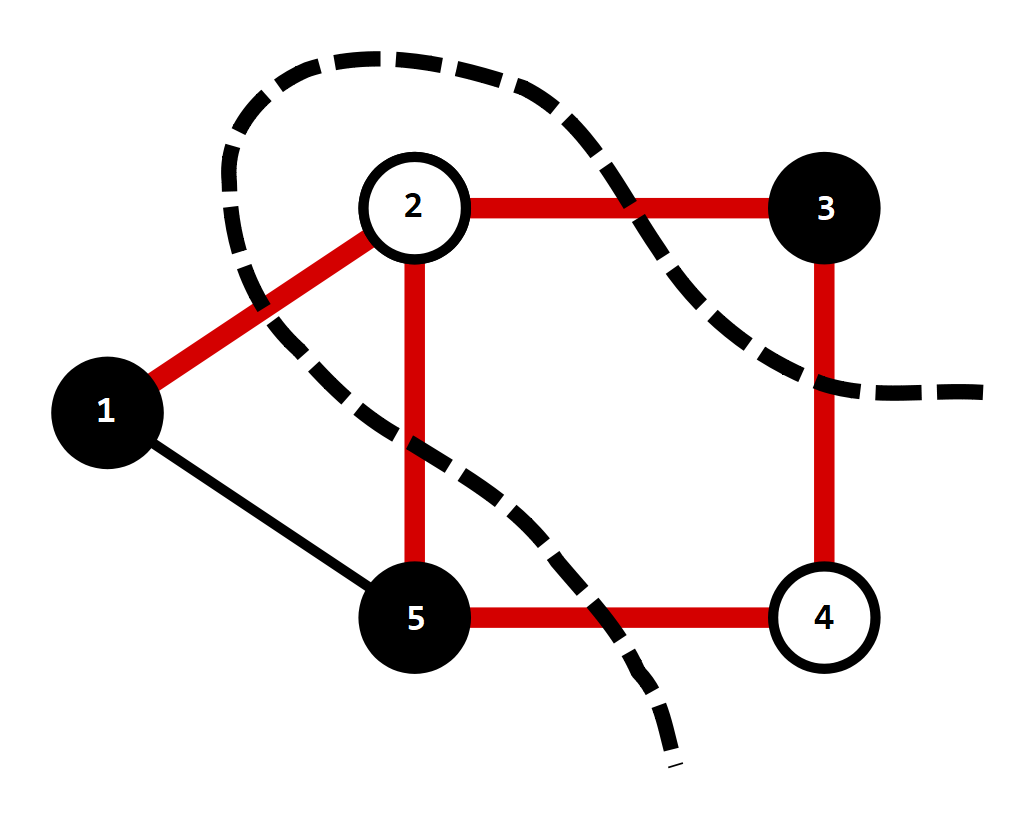
\includegraphics[width=0.5\textwidth]{figures/MaxCut.png}
	\caption{An example of the Max-Cut problem on a graph with 5 nodes. The nodes are partitioned into two sets; black nodes and white nodes. The goal is to maximize the number of edges between the two sets (these are colored red). More generally when talking about weighted graphs we want to maximize the sum of the weights of the edges connecting the two sets. Figure from \cite{wiki:MaxCut}}
	\label{fig:MaxCut}
\end{figure}

For reasons that will become apparent in Chapter \ref{chap:qaoa}, it is sometimes useful to write the bipartition in terms of a bit string. A bit string is simply a sequence of bits, usually denoted by $0$ or $1$. This can be achieved by labelling the $n$ vertices in a particular order $(1, \dots, n)$. By using the fact that the partition is completely characterized by \emph{one} set $S$, we can represent a partition of $V$ into $S$ and $\bar{S}$ by a bit string $\vec{x}$ consisting of ones and zeros. We can translate between the two using the function $f: \mathcal{P}(V) \mapsto \{0,1\}^{n}$ defined by
\begin{equation}
	f(S) = \big(\mathbf{1}_S(1), \dots, \mathbf{1}_S(n) \big)
\end{equation}
where $\mathcal{P}(V)$ denotes the powerset of $V$, and $\mathbf{1}_{S}$ denotes the characteristic function of $S$. For example, let us label the vertices in Figure \ref{fig:MaxCut} in clockwise fashion starting from the leftmost vertex. We can represent the cut shown as $\vec{x} = (1,0,1,0,1)$, where the black nodes constitute set $S$ and the white nodes consitute set $\bar{S}$. The objective function in terms of $\vec{x}\in \{0,1\}^n$ becomes
\begin{equation}
C(\vec{x}) = \sum_{\{i,j\} \in E} w_{i,j}(x_i-x_j)^2
\label{eq:maxcut bitstring objective}
\end{equation}
Equivalently, we can use a binary string $\vec{z} \in \{-1,1\}^n$. The objective function is then described by
\begin{equation}
	C(\vec{z}) = \sum_{\{i,j\} \in E}\frac{w_{i,j}}{2}(1-z_iz_j)
\end{equation}
This approach will become useful in the next chapter, where we will talk about spins.

\newpage
\section{Approximation algorithms and ratios}
% NP complete
The Max-Cut problem is an example of a problem that is NP-complete \cite{Karp72}. NP-completeness implies NP-hardness which roughly means we have to resort to extensive searching in order to find the optimal cut. To be more precise, no polynomial-time algorithms for Max-Cut are known for arbitrary graphs. Therefore, we have to resort to finding good solutions instead. One approach to find such good solutions is to design approximation algorithms. These algorithms seek to find solutions that guarantee the objective value to be at least the optimum times a certain ratio, called the approximation ratio $\rho$.
\begin{equation}
\frac{C(\vec{x})}{C_{\max}} \geq \rho
\end{equation}
where $C_{\max} = \max_{\vec{x}} C(\vec{x})$. Note that $\rho \leq 1$ as we can not do better than the optimal solution. Note that these algorithms grant a guarantee that the objective value for a found solution $\vec{x}$ lies in a particular range
\begin{equation}
\rho C_{\max} \leq C(\vec{x}) \leq C_{\max} 
\end{equation}
It certainly might be the case that for particular instances of the problem an approximation algorithm finds solutions that are better than $\rho C_{\max}$.

\subsection{Bounds on the approximation ratio of Max-Cut}
In 2002 the Swedish theoretical computer scientist H\r{a}stad proved that it is NP-hard to approximate the Max-Cut value with an approximation ratio better than $\frac{16}{17} \approx 0.941$  for Max-Cut on all graphs \cite{Hastad02}, or $331/333 \approx 0.994$ when restricted to unweighted 3-regular graphs \cite{BK99}. As the approximation ratio for polynomial-time algorithms for Max-Cut is bounded, this means that the problem is in the class APX, for approximable problems.

In addition, there is a conjecture from theoretical computer science called the Unique Games Conjecture (UGC) \cite{UGC}. The conjecture postulates that the problem of determining the approximate value of a unique game, is NP-hard. The details of the Unique Games Conjecture are rather technical and not relevant for the rest of this work, I refer the interested reader to the original paper \cite{UGC}, or to \cite{UGC-Blog} for a less formal discussion. However, there is a consequence of the conjecture that is relevant. It turns out that if the UGC is true, then there exists no polynomial time algorithm that can beat Goemans-Williamson \cite{KKMO05}, thus restricting the possible approximation ratio even further to around $0.878$. 

At the moment, it is unknown whether or not the conjecture is true, but it is interesting to note that an approximation algorithm that is better than Goemans-Williamson would imply that the UGC is false. Unlike the question whether or not $P = NP$, currently there seems to be no consensus in the academic world around the Unique Games Conjecture.

\section{Classical Algorithms for Max-Cut}
In this section I will discuss known classical algorithms for solving Max-Cut to give a sense of what is already possible on classical computers. The presentation of the algorithms in the coming subsections largely follows the structure of \cite{lecture-MaxCut, lecture-GW}.
\subsection{Greedy approach}
One algorithm for solving Max-Cut uses a greedy approach and guarantees an approximation ratio of $\frac{1}{2}$. 

Let $G(V,E)$ be an undirected graph with edge weights $w_e$ for $e\in E$ and label $V = \{1, \dots n\}$ so there is some ordering. Next, define $E_i = \{(k,i) : \{k,i\} \in E, k < i\}$, the set of edges entering vertex $i$ from ``lower'' nodes. Note that $E_i \cap E_j = \emptyset$ if $i \neq j$ because of the strict inequality. Initially, set $S = \{1\}$ and $\bar{S} = \emptyset$.  Then starting from $i=2$, add node $i$ to either $S$ or $\bar{S}$ so that the sum of the number of edges in $E_i$ that are in the cut times their respective weights is maximized. Increment $i$ and repeat the last step until $i=n$.

As an example, consider the graph from Figure \ref{fig:MaxCut}. For simplicity I will consider it to be an unweighted graph with $w_{i,j} = 1$ for all $\{i,j\}\in E$. Starting with $S = \{1\}$, consider node $2$. We choose to add node $2$ based on what choice maximizes $\sum_{e \in E_2 \cap K(S)}w_e$, which in our case is simple: we add node $2$ to set $\bar{S}$ because then edge $(1,2)$ is in the cut. We move on to node $3$ with $E_3 = \{(2,3)\}$, and we choose node $3$ to be in $S$ because then edge $(2,3)$ is in the cut. Analogously, we add edge $4$ to $\bar{S}$. Node $5$ is somewhat more tricky as we have $E_5 = \{(1,5),(2,5),(4,5)\}$ containing 3 edges instead of just one. Adding node $5$ to $S$ would yield $\sum_{e \in E_5 \cap K(S)}w_e = 2$ while adding it to $\bar{S}$ would yield $\sum_{e \in E_5 \cap K(S)}w_e = 1$. Therefore, we add node $5$ to $S$ and we are done. The final result is thus $S = \{1,3,5\}$ and $\bar{S} = \{2,4\}$ with a cutvalue of 5, which is actually optimal.
\\

Let us proof that this is indeed an approximation algorithm with approximation ratio $\frac{1}{2}$. Define $K$ to be the cut obtained by the algorithm, and observe that $E_1, \dots E_n$ is a partition of $E$ as the sets are pairwise disjoint and $E = \bigcup_i E_i$. For each node $i \in V$, define $\tilde{E}_i = E_i \cap K$. Note that the cut $K$ is the union of these newly constructed sets $K = \bigcup_i \tilde{E}_i$. The finalizing observation is that we chose $S,\bar{S}$ in such a way that 
\begin{equation}
\sum_{e\in \tilde{E}_i}w_e \geq \frac{1}{2}\sum_{e \in E_i}w_e \qquad \forall i \in V
\end{equation}
Therefore we have that 
\begin{equation}
	C(S) = \sum_{i\in V} \sum_{e \in \tilde{E}_i} w_e \geq \frac{1}{2}\sum_{i\in V} \sum_{e \in E_i} w_e = \frac{1}{2}\sum_{e\in E} w_e \geq \frac{1}{2}C_{\max}
\end{equation}
where the latter inequality is derived from the fact that the optimum cut can not be larger than the sum of the weights of all edges.

\subsection{Random partition}
\label{sec:random-partition}
Another algorithm for solving Max-Cut that is quite easy to implement is simply choosing a random partition. As the name suggests, it is a stochastic algorithm. 

Let $G = (V,E)$ again be an undirected graph. We choose each vertex in $V$ to be in either $S$ or $\bar{S}$ with equal probability $\frac{1}{2}$. This bipartition defines a cut $K(S)$, whose expected size we will now calculate. 

Consider an edge $e \in E$ in the graph. Remark that $\prob{e \in K(S)} = \frac{1}{2}$. For $e \in E$, we define $\chi_e$ to be a random variable such that $\chi_e = 1$ if $e \in K(S)$ and $\chi_e = 0$ if $e \notin K(S)$. The value of the cut is then
\begin{equation}
	C(S) = \sum_{e\in E} w_e\chi_e
\end{equation}
Note that the value itself is now a random variable, so we have to resort to calculating the expecation value of the cut. Using linearity of the expectation operator, we obtain the following
\begin{equation}
	\expect{C(S)} = \sum_{e \in E} w_e\expect{\chi_e} = \sum_{e \in E}w_e \prob{e \in K(S)} = \frac{1}{2}\sum_{e \in E}w_e \geq \frac{1}{2}C_{\max}
\end{equation}
Resulting in a $\frac{1}{2}$-approximation ratio in expectation. I would like to emphasize that we give a lower bound for the expectation value of the objective function, and not a lower bound for every outcome. Note that it might be the case that the algorithm produces with probability $2^{-n}$ a partition $S = V, \bar{S} = \emptyset$ with a cutvalue of 0. 

\subsection{Goemans-Williamson}
The best classical approximation algorithm for solving Max-Cut known is the algorithm proposed by Goemans and Williamson (GW) in 1994 \cite{GW95}. The algorithm is also stochastic and has an approximation ratio $\rho \approx 0.878$ in expectation. Prior to GW, the best-known approximation algorithms for the Max-Cut problem had performance guarantee of $\frac{1}{2} + o(1)$, meaning that the achieved approximation ratio is below $\frac{1}{2} + \epsilon$ for any $\epsilon>0$. The GW-algorithm was indeed quite a breakthrough. 

The algorithm uses a sophisticated method that randomly rounds the solution to a nonlinear programming relaxation. Before I will present the algorithm, the following two definitions are useful.

\begin{definition}
	A square $n \times n$ matrix $A$ is called \textbf{positive semidefinite} if the following holds
	\begin{equation}
	\vec{x}^TA \vec{x} \geq 0 \qquad \forall \vec{x} \in \mathbb{R}^n
	\end{equation} 
	This property is sometimes indicated using $A \succcurlyeq 0$
\end{definition} 

\begin{definition}
	 A \textbf{semidefinite program} is the problem of optimizing a
	linear function of a symmetric positive semidefinite matrix subject to linear equality constraints.
\end{definition}
Indeed a semidefinite program is a subclass of the more general linear programs, so it is possible to solve these using the well known Simplex method \cite{simplex}. While the Simplex method itself is not a polynomial time algorithm, it can be generalized to semidefinite programs \cite{pataki}. Given any $\epsilon >0$ these semidefinite programs can be solved in polynomial time within an additive error of $\epsilon$. This can be done using a variety of methods, these include interior point methods \cite{nesterov1994interior}, the ellipsoid method \cite{lovasz1988geometric}, and other polynomial-time algorithms for convex programming \cite{vaidya}.

The problem to be solved is

\begin{maxi!}|l|
	{\vec{z}}{\frac{1}{4}\sum_{\{i,j\}\in E}w_{i,j}(z_i-z_j)^2}
	{}{}
	\label{probleem1}
	\addConstraint{z_i \in \{-1,1\} \text{ for } i \in V}
	\label{probleem2}
\end{maxi!}
which is equivalent to what we saw in \eqref{eq:maxcut bitstring objective}.
Let us denote the optimal solution of this program as $C_{\max}$. Next, we introduce a \emph{relaxation} of the problem meaning that we let loose of some of the constraints in order to make solving it easier
\begin{maxi!}|l|
	{\vec{z}}{\frac{1}{4}\sum_{\{i,j\}\in E}w_{i,j}(\vec{y}_i\cdot \vec{y}_i + \vec{y}_j\cdot \vec{y}_j - 2\vec{y}_i\cdot \vec{y}_j)}
	{}{}
	\addConstraint{\vec{y}_i \in \mathbb{R}^n \text{ and } \|\vec{y}_i\|^2 = 1 \text{ for } i \in V}
\end{maxi!}
Note that the above problem is indeed a relaxation, as we can simply take $\vec{y}_i = z_i \vec{e}_1$ to reconstruct program \eqref{probleem1}, \eqref{probleem2}, where $\vec{e}_1$ is the first standard basis vector of $\mathbb{R}^n$. Let me denote the optimal solution of the relaxation as $\tilde{C}_{\max}$, then we have $\tilde{C}_{\max} \geq C_{\max}$. The above so called vector program is equivalent to the following semidefinite program, where we define a matrix $A = (a_{ij})$
\begin{maxi!}|l|
	{\vec{z}}{\frac{1}{4}\sum_{\{i,j\}\in E}w_{i,j}(a_{ii}+a_{jj}-2a_{ij})}
	{}{}
	\addConstraint{a_{ii} = 1 \text{ for } i \in V \text{ and } A \succcurlyeq 0} \text{ and symmetric}
\end{maxi!}

This semidefinite program can be solved in polynomial time obtaining an optimal matrix $A^*$ with value $c$. Note that the solution could be irrational. In that case we can find an approximation that is rational in polynomial time with value $c'$ with $c - \epsilon < c' < c$ for any $\epsilon > 0$. Using the symmetry of the semidefinite matrix $A^*$ we know that we can decompose $A^* = U^TU$ where $U$ is an $m \times n$  matrix with $m \leq n$, this is called the Cholesky decomposition. Next, we consider the column vectors of $U = \{\vec{u}_1,\dots \vec{u}_n\}$. Because of the semideniteness of $A^*$ and the constraint that $a_{ii}^* =1$, we know that these are unit vectors $\|\vec{u}_i\|^2 = \vec{u}_i^T\vec{u}_i = a^*_{ii} = 1$. Moreover, we know that $\vec{u}_i \in \mathbb{R}^m$ for $i = 1, \dots, n$ and since $m \leq n$ we can embed these vectors in $\mathbb{R}^n$. Thereafter, we randomly choose a hyperplane through the origin, and in polynomial time we can figure out which vectors are above or below the hyperplane. The vectors $\vec{u}_i$ that lay above the plane denote vertices that are on one side of the partition, and the vectors $\vec{u}_i$ below the plane denote the vertices that are on the other side of the partition.

Using a combination of geometric arguments and insights from calculus, it can be shown that the algorithm has an approximation ratio of 
\begin{equation}
\rho = \frac{2}{\pi} \min_{0 \leq \theta \leq \pi} \frac{\theta}{1 - \cos \theta}
\end{equation}
in expectation, which numerically evaluates to $\rho \approx 0.878$ \cite{GW95}. 

For a more extensive discussion of the Goemans-Williamson algorithm I refer to \cite{GW95,GW-lecture-Hollbach,lecture-GW}.

\section{Applications of Max-Cut}
The maximum cut problem is a natural and simple to understand graph problem often discussed in introductory optimization or algorithm courses. There are also some applications of the problem. An example of which is efficient design of electric circuits or communication networks \cite{wang2010maximum}, but the problem also has uses in statistical physics, namely in finding the groundstate energy in spin glass \cite{maxcut-applications}.

\subsection{Ising Model} %maybe a paragraph is more suitable
The Ising model describes a system of $n$ particles with two possible states, for example spin up and down. See Figure \ref{fig:ising-model} for an illustration. The system can then be characterized by a binary string $\sigma \in \{-1,1\}^n$. Following the example, $1$ denotes spin up and $-1$ denotes spin down. The Hamiltonian reads as follows
\begin{equation}
H(\sigma) = \sum_{\{i,j\}} J_{ij} \sigma_i \sigma_j - \mu \sum_i h_i \sigma_i 
\end{equation}
where the first sum is over the adjacent pairs $\{i,j\}$ in the system, and $J_{ij}$ designates the strength of the interaction of the constituents of that pair. The second sum describes the interaction with some magnetic field, with strength $h_i$ at site $i$. Note that when there is no external magnetic field, i.e. $h_i = 0$ for all $i$, then the problem of finding a groundstate is equivalent to the Max-Cut problem. Closely related to the Ising model is the Sherrington-Kirkpatrick model. 

\begin{figure}[H]
	\centering
	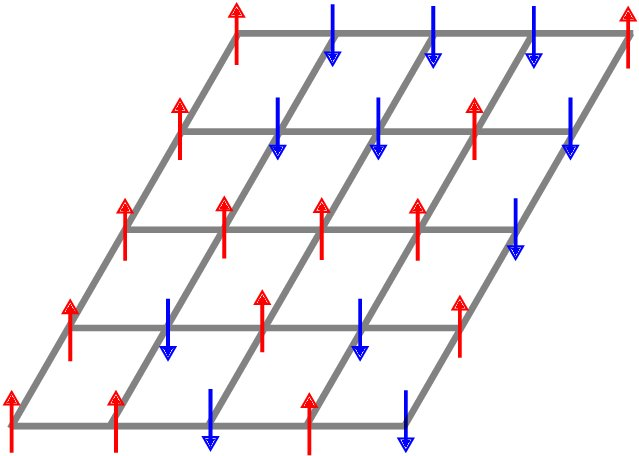
\includegraphics[width=0.5\textwidth]{figures/Ising-model-on-a-square-lattice.jpg}
	\caption{Schematic representation of a configuration of the 2D Ising model on a square lattice. Figure and caption from \cite{ising-model}}
	\label{fig:ising-model}
\end{figure}